This was the strongest result in the project. Across four runs the anchored estimator had lower
inter-seed IQR in 19/20, 21/23, 25/27 and \textbf{15/16} comparisons (primary set: \(p = 5.2 \times 10^{-4}\),
median ratio \textbf{13.5x, 95\% CI 4.6--20.7}, n = 16), with a clean dose--response between the
selected weight and the effect:
\textbf{Spearman $\rho$ = +0.585, \(p = 4.1 \times 10^{-9}\), n = 85}.

\begin{figure}[t]
\centering
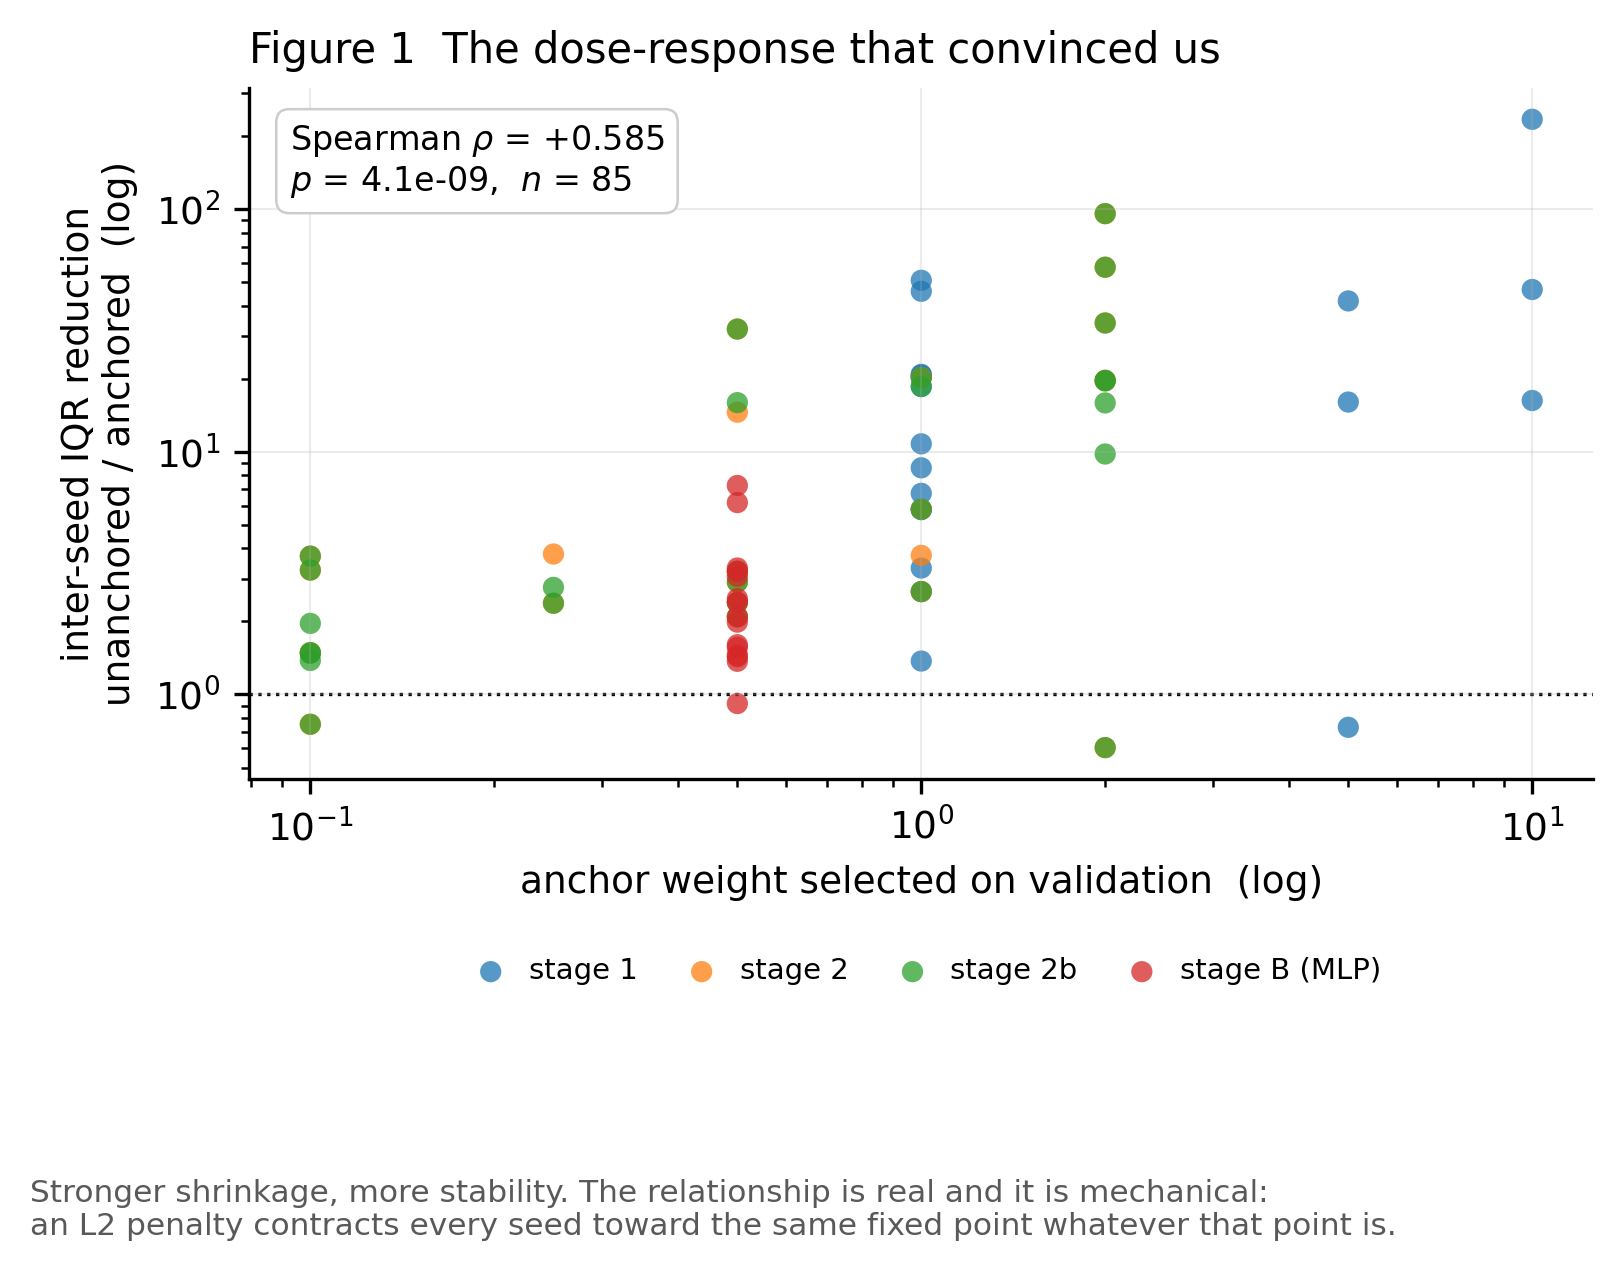
\includegraphics[width=\linewidth]{figures/figure1_dose_response.png}\label{fig:dose}
\caption{Figure 1}
\end{figure}

\textbf{Figure 1 is reproduced because we ourselves found it persuasive.} It is the evidence that
convinced us, pooled across all four runs, and it is an artefact. Its apparent strength
illustrates how easily this failure mode survives conventional statistical scrutiny --- which is
the difficulty the rest of the section is about.

An L2 penalty pulls every seed toward the \emph{same fixed target}. As the weight grows all seeds
converge on that target and inter-seed dispersion goes to zero \textbf{by construction} --- whatever
the target is. The dose--response we took as corroboration is the signature of the artefact.

\textbf{The control.} Re-run with the real prior \textbf{permuted in time}: identical mean, standard
deviation and marginal distribution; correlation with tomorrow's absolute return 0.0007 versus
0.041. Matched on magnitude, stripped of information.

\begin{longtable}[]{@{}llll@{}}
\toprule
ticker & weight & real prior & shuffled prior\tabularnewline
\midrule
\endhead
NVDA & 0.5 & 1.55$\times$ & 1.49$\times$\tabularnewline
NVDA & 1.0 & 2.25$\times$ & \textbf{2.91$\times$}\tabularnewline
SQM & 0.5 & 0.76$\times$ & 0.63$\times$\tabularnewline
SQM & 1.0 & 1.33$\times$ & 1.15$\times$\tabularnewline
\^{}GSPC & 0.5 & 3.05$\times$ & \textbf{3.10$\times$}\tabularnewline
\^{}GSPC & 1.0 & 12.47$\times$ & \textbf{16.76$\times$}\tabularnewline
\bottomrule
\end{longtable}

The uninformative prior matches or beats the real one in 3 of 6 cells; \textbf{Wilcoxon \(p = 0.844\)}.
Bootstrapped over comparisons, the two are indistinguishable: real prior \textbf{1.9x (95\% CI
1.0--7.8)} against shuffled \textbf{2.2x (95\% CI 0.9--9.9)}. The intervals overlap almost entirely,
which is a more informative statement of the null than the rank test alone.

\emph{Control: shrink toward a scale-matched nonsense target. Cost: 28 minutes, validation only,
zero test-set evaluations.}

\textbf{A trap.} Pooling all controls gives 1.32$\times$ against 2.36$\times$ for informative priors, which looks
like a genuine gap. It is produced entirely by a control shrinking toward an off-scale target,
which fights the data rather than shrinking within it. Only the \textbf{scale-matched} comparison is
diagnostic, and it is null. Reporting the aggregate would have preserved the claim.

\textbf{This is a restricted randomization test, and we should have known that before running it.}
The requirement we arrived at by tripping over the trap above --- that the permuted target must
preserve the properties irrelevant to the hypothesis and destroy only the one under test --- is
stated directly by Ojala and Garriga (2010), whose second permutation test permutes features
within classes for exactly this reason: \emph{each randomization method entails a certain null
distribution, that is, which properties of the original data are preserved.} An off-scale
control induces a different null and is therefore not diagnostic. We report the sequence
honestly --- we found the constraint empirically and located its name afterwards --- because the
control is more credible with a seventy-year lineage (Fisher 1935; Pitman 1937) than as an
invention of ours.
